% !TEX root =  ../thesis.tex
\section{Privacy awareness context}
We now define the scope of this thesis, going through the main factors affecting privacy in mobile applications, and describing the existing relationships between them.

We identify three main factors to take into consideration:
\begin{itemize}
  \item permissions
  \item actions and behaviors
  \item privacy policies
\end{itemize}

\emph{Permissions} determine which data or services the app can access on the user's device, so they effectively define the maximum potential impact an application can have over the user's privacy: the fewer the permissions, the lower the risk. However, a recent study \cite{stickley} showed how, given only the \texttt{INTERNET} permission, an Android application was capable of stealing online account login credentials.
This highlights how permissions only represent a loose upper bound to the risk: even apps requesting one single permission can significantly affect the privacy of user.

% As discussed in \autoref{sec:android-permission-model}, permissions are declared upfront by Android applications and they are visible prior to the app's installation.

We define \emph{actions} as the minimum unit of work an application can do. Actions can be divided in two main categories

\begin{itemize}
  \item actions that cannot be performed without an explicit permission, and actions
  \item that do not require such explicit permission (e.g. impact local state of app)
\end{itemize}
The former category typically includes actions that have any impact on the device's security. Such actions are forbidden by the OS (\emph{Operating System}) by default, and are allowed only if specific permissions have been granted to the application. The latter usually represents actions not affecting the device's security, e.g. actions confined within the bounds of the application's internal logic.

We define \emph{behaviors} as sequences of one or more actions; such definition implies that some behaviors, namely those including actions from the first category, can occur only when specific permissions have been granted.


\begin{example}
\leavevmode
Let us a consider a game application that stores user's top scores and sends them over the Internet to a remote server.
We can break this app down into the following actions:
\begin{itemize}
  \item \texttt{save\_user's\_top\_scores} ($A_1$)
  \item \texttt{send\_top\_scores\_over\_the\_internet} ($A_2$)
\end{itemize} 
The sequence of $A_1$ and $A_2$ forms the behavior \texttt{store\_and\_send\_user's\_ top\_score\_to\_a\_ remote\_sever} ($B_1$).
$A_2$ requires the permission \linebreak \texttt{INTERNET} to be granted, whereas $A_1$ can always be performed.
This implies that $B_1$ can occur only if permission \texttt{INTERNET} is granted.
\end{example}

Thus, permissions enable actions, and actions can be composed to form behaviors. It is important to notice the cardinality of these relationships: one permission enables one or more actions; in turn, a behavior is enabled by one or more actions.

A many-to-many relationship exists between permissions and behaviors. Enabling one (or more) permissions can potentially enable one or more behaviors.
While some of these behaviors are expected, and even desirable, some others might result unexpected and potentially undesirable. 

\begin{figure}[tb]
\centering
     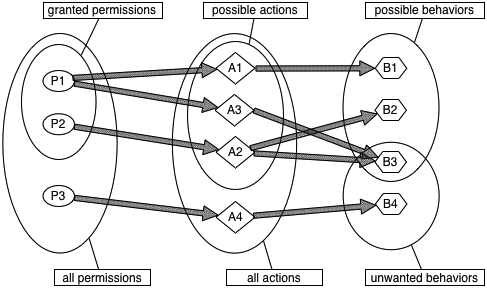
\includegraphics[width=0.9\textwidth]{images/context}
      \caption{Relationships between permissions, actions and behaviors}
      \label{fig:privacy-context}
\end{figure}

\autoref{fig:privacy-context} exemplifies this possible scenario: permission $P_1$ is required to enable action $A_1$ which in turn enables behavior $B1$. Similarly, permission $P_2$ enables action $A_2$ and consequently behavior $B_2$. Granting permissions $P_1$, however, also enables action $A_3$, and when combined with action $A_2$, an unwanted behavior $B_3$ may occur.

A practical instance of this scenario is the following:
\begin{example}
\leavevmode
\label{ex:unwanted-behavior}
\begin{itemize}
  \item the \texttt{READ\_PHONE\_STATE} permission enables the action \texttt{detect\_an\_ incoming\_phone\_call} ($A_1$), which enables the behavior \texttt{pause\_ the\_game\_when\_an\_incoming\_phone\_ call\_arrives} ($B_1$).
  \item the \texttt{INTERNET} permission enables the action \texttt{\justify send\_and\_receive\_ data\_over\_the\_Internet} ($A_2$), which enables the behavior \texttt{send\_ the\_user's\_top\_score\_to\_a\_remote \_server} ($B_2$).
  \item the \texttt{READ\_PHONE\_STATE} permission also enables the action \texttt{read\_the\_ user's\_phone\_ number} ($A_3$). The combination of actions $A_2$ and $A_3$ enables the behavior \\ \texttt{send\_the\_user's\_phone\_number\_to\_a\_remote\_server}($B_3$), which may be undesirable.
\end{itemize} 
\end{example}

Since the permission-based model has such shortcomings in properly restricting actions and avoiding unwanted behaviors, privacy policies are commonly provided together with the application, acting as a supplementary filter on the possible behaviors, telling the final users which of the possible behaviors the app is going to actually generate.

Coming back to Example 2, a privacy policy may explicitly state that the user's phone number is never collected nor accessed, promising the application will never perform \emph{A3}, and hence ruling out \emph{B3}. Nonetheless, nothing forbids an app to deviate from its policy.

\section{Scope of this thesis}
This thesis work focuses on the first two steps discussed in the previous section.

The first step requires an in-depth analysis and comprehension of the most requested permissions, in order to identify the potential privacy concerns each one of them carries.

Once the permissions of interest have been identified we then perform a manual analysis in order to understand how privacy policies deal with the privacy concerns represented by them. The manual analysis will enable an automated process, which, given an arbitrary Android application published on the Play Store platform, retrieves its privacy policy and produces a human-readable report about the relationships between the permissions list and the analyzed legal document.

The final result will then allow a potential user to aggregate a large amount of privacy-related information in a quick and concise way, marking a clear step towards privacy awareness.

%%%%%%%%%%%%%%%%%%%%%%%%%%%%%%%%%%%%%%%%%%

\section{Scope and goals of this thesis}
This thesis describes a methodology, supported by tools, that enables a user who installs an Android application to gain a better understanding of the app's capabilities, based on the permissions it requires and its privacy policy, and alerts the user to some of the (potentially) unintended consequences that the user grants the application by installing it.

\todo[inline]{Blablabla}
\section{Steps towards privacy awareness}
Given the general context of privacy awareness, we now identify a set of steps we intend to follow in our work, aiming at producing an increased users' awareness.

\begin{enumerate}
  \item Understanding permissions \hfill \\
    Previous studies \cite{Felt:2012:APU:2335356.2335360} show how permissions are rarely understood by users. Specifically users appear not be able to correlate a permission with the possible actions it enables, let alone the spectrum of possible behaviors derived from actions interleaving.

    The first step towards awareness is to analyze permissions and derive potential consequences. We are especially interested in permissions that directly affect privacy. As an example, the \texttt{READ\_PHONE\_ STATE} permission is typically requested by apps in order to be able to respond to phone events such as a incoming call, but it also enables the app to read the user's phone and IMEI numbers.

    Once permissions have been fully analyzed, one can then identify their  effect on the user's privacy.

  \item Correlating permissions and privacy policies \hfill \\
    The next step towards privacy awareness is to map each permission the app requests into its impact, as stated in its privacy policy.
    While privacy policies do not share a common defined structure, they do express similar concepts in similar ways, which allows us to extracting useful pieces of information from them. For example, an application requesting the \texttt{ACCESS\_FINE\_LOCATION} permission is very likely to be associated to a privacy policy containing expressions such as \emph{``GPS'', ``Location Services'', `Global Positioning System', etc}.

    This step takes into consideration each permission that enables an app to affect the user's privacy, with the final goal of building a dictionary of common expressions and patterns that associate the permission to natural language sentences in the privacy policy.

  \item Correlating apps behavior and privacy policies \hfill \\
    The final step is to monitor the app's actual behavior. Recalling Example \ref{ex:unwanted-behavior}, the application might never retrieve the user's phone number even though it requested such permission.

    On this basis we can advise the users about how well an application with respects the claims expressed in the privacy policy, and the actual actions taken by the app once installed and running on their phone.
\end{enumerate}

\begin{figure}[tb]
\centering
     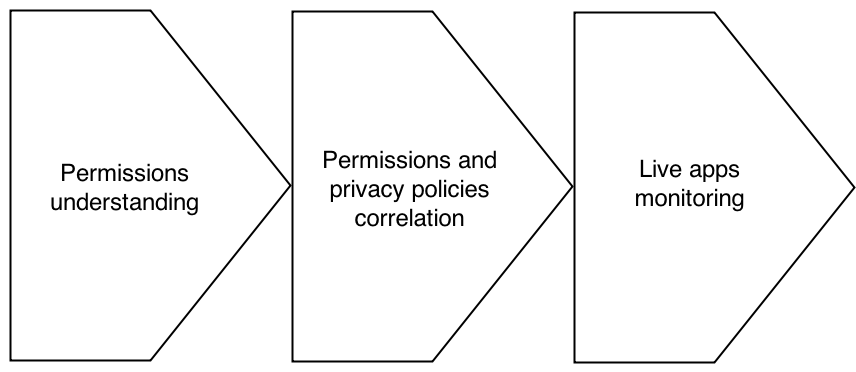
\includegraphics[width=0.8\textwidth]{images/awareness-steps}
      \caption{Privacy awareness steps}
      \label{fig:awareness-steps}
\end{figure}

%%%%%%%%%%%%%%%%%%%%%%%%%%%%%%%%%%%%%%%%%%

\section{Android OS Permission Model}
\label{sec:android-permission-model}
As explained in the Android Developer Guide, ``Android is a privilege-separated operating system, in which each application runs with a distinct system identity. [...]
Additional finer-grained security features are provided through a permission mechanism that enforces restrictions on the specific operations that a particular process can perform, and per-URI permissions for granting ad-hoc access to specific pieces of data. [...]
A basic Android application has no permissions associated with it by default, meaning it can not do anything that would adversely impact the user experience or any data on the device.''\cite{android-developer-guide}.
In order to access the protected features of the device the developer has to declare a list of permissions the application needs. This list is specified in the \texttt{AndroidManifest.xml}, a file containing application metadata, included by every Android application.

For example, an application that needs to send and receive data over the Internet would specify an \texttt{AndroidManifest} similar to the one in \autoref{lst:manifest}.

\begin{lstlisting}[
caption=Example of permission declaration in AndroidManifext.xml,
language=XML,
backgroundcolor=\color{white},
label=lst:manifest,
frame=single,
float,
basicstyle=\ttfamily\footnotesize
]
<manifest xmlns:android="http://schemas.android.com/res/android"
    package="com.example.anapp" >
    <uses-permission android:name="android.permission.INTERNET"/>
    ...
</manifest>
\end{lstlisting}

``At application install time, permissions requested by the application are granted to it by the package installer, based on checks against the signatures of the applications declaring those permissions and/or interaction with the user.
No checks with the user are done while an application is running: it either was granted a particular permission when installed, and can use that feature as desired, or the permission was not granted and any attempt to use the feature will fail without prompting the user.''\cite{android-developer-guide}

%%%%%%%%%%%%%%%%%%%%%%%%%%%%%%%%%%%%%%%%%%
\section{Related Work}
As discussed in \autoref{sec:android-permission-model}, permissions are granted at install time, meaning that a user is supposed to have reviewed the permissions the application requested and to have deemed them acceptable, before granting them altogether.

Such mechanism has been criticized for several reasons: first of all, recent studies \cite{Felt:2012:APU:2335356.2335360} \cite{Kelley:2012:CPI:2426020.2426027} show how users might not have complete understanding of the meaning and consequences of each permission in the list. The same studies also show how even experienced users are found not to pay attention to the permission list, most likely due to its verbosity and length. To further prove this last observation, in a recent experiment \cite{stickley} an ad-hoc application was developed and put on the Play Store; the application requested all possible permissions, enabling the researchers to steal personal data from the user, such as email addresses and phone numbers. The application received 1300 downloads over a 3-month period, without being advertised, and collected 1950 email addresses.

%%%%%%%%%%%%%%%%%%%%%%%%%%%%%%%%%%%%%%%%%%